%!TEX root = thesis.tex

\chapter{Introduction}
\label{ch:intro}

\section{Background}
\subsection*{Human-Computer Interaction}
Human-Computer Interaction (HCI) is limited in transmission rate. The information per second rate is still low nowadays, and innovation is progressing slowly. Since the introduction of the mouse in the seventies very few revolutionary new and still affordable peripherals where introduced that aid the communication with a computer. The most notable innovations in HCI are the Wii - which is mainly used for gaming - and (multi) touch screen, which is becoming more popular for integration smartphones.

\begin{figure}[htbp]
	\center{}
	\label{fig:mouse}
	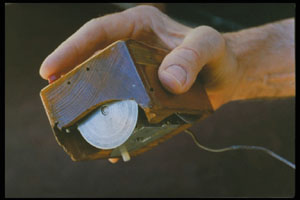
\includegraphics[width=0.3\linewidth]{figures/mouse.jpg}
	\caption{The first mouse}
\end{figure}

New and revolutionary ideas are required to create new peripherals that improve productivity, but are still intuitive and thus easy to learn to use. To get inspiration for improvement, one can look around and study already existing communication methods, for example the communication between humans. 

When two people are in a room and don't have a audio or visual limitation, they will probably communicate by speech. But there is much more going on than only producing and interpreting words. The intonation, speed and other small variations in the voice add a lot more information to the words. Also the facial expression and body language give more space for expression. Some people like to 'talk with their hands' while telling a story, something that adds more expression to the transmitted information.

\subsection*{Sign Language}

A deaf person can't interpret spoken words, at least not by listening. He or she is highly depended on visual information. Sign languages have been emerged or invented to aid this visual communication. In these languages two elements have an important role, the face and the hands. These body parts give the most expressive power. The face because it is very good for expressing feelings and emotions, and the hands because they are very deformable. This makes the hands very interesting and useful, since there are countless combinations of finger poses and orientations. 

Speech generation, speech recognition, facial expression recognition and sign language interpretation are all subject of extensive research at the moment. Breakthroughs in these area's are important for revolutionary new interfaces which can tremendously improve the speed of interaction and usability for a user. 

In this thesis I want to look into the details of using computer vision to interpret sign language and especially to use sign language to actually control the computer - to use your hands for non-intrusive interaction. To show the advantages of having such a system I wanted to find an application for it and demonstrate that this can be actually useful. The application I found was sound generation and manipulation, or said differently; making music. 

Translating sign language into music is a very interesting concept, not only because it sounds poetic but it can really demonstrate the power of such a system. Making life music is a complex process where real-time interaction between a artist and his tools is important. Also, for an audience it is much more compelling to look at a artist who is physically more active than only clicking a mouse.

\subsection*{Hand Poses}
Studying sign language brought the understanding that there are not really signs for musical concepts. Usually when music is translated into sign language only the vocals are translated. Facial expression and references to emotions are used to indicate the 'mood' of the music and the speed and expressiveness of the gestures indicate the intensity of the music, but these kind of gesture are not really usable for HCI because they are too subjective. A more formal method is required. Also, previous studies have shown that the segmentation of the consecutive gestures is a difficult task\cite{Buehler2009}.

It is more feasible to have a limited set of hand poses that corresponds to a set of commands and parameters.  Any set of hand poses would do for this system, as long as the individual poses don't look too similar.  But since the idea is to translate the interpreted hand poses into sound, it would be interesting to use a set of poses that has a already existing relationship to sound.

In Medieval music, the Guidonian hand was a mnemonic device used to assist singers in learning to sight sing. The idea of the Guidonian hand is that each portion of one hand represents a specific note within the hexachord system, which spans nearly three octaves. The other hand is used to point to the correct hand portion. \autoref{fig:guidonian} shows a hands with the tonal positions.

\begin{figure}[htbp]
	\centering{}
	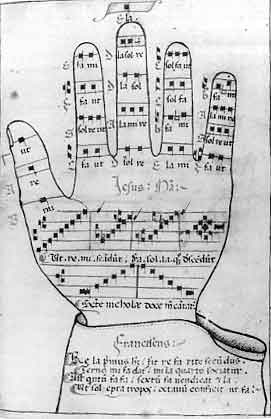
\includegraphics[width=0.3\linewidth]{figures/guidonian_hand.jpg}
	\caption{Guidonian Hand}
	\label{fig:guidonian}
\end{figure}

Despite the fact that this system has a large set of symbols - 22 to be exact - this system is not usable since the individual poses are very much alike. Discriminating between the different poses will probably be problematic.

A more recent method using hand poses in relation to music are the Curwen solfege hand signs\cite{choksy1999}. This method was introduced in the 19th century by John Curwen, who also is the founder of the famous tonic sol-fa. The tonic sol-fa is better known as \emph{'do re mi fa sol la ti'}.

\begin{figure}[htbp]
	\centering{}
	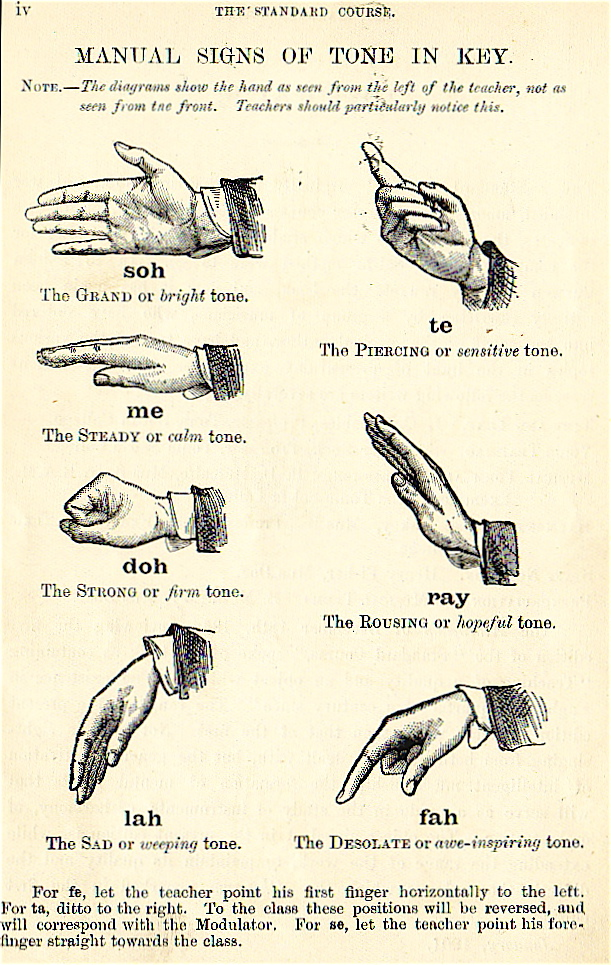
\includegraphics[width=0.4\linewidth]{figures/curwen.jpg}
	\caption{Depiction of Curwen's Solfege hand signs from 1904}
	\label{fig:curwen}
\end{figure}

\autoref{fig:curwen} is a scan from a teaching book from 1904 where the 6 tonal hand poses are shown. These 6 poses correspond to the 6 notes in the musical major scale. These hand poses are much more suitable for our system, since the individual hand symbols are distinct. Also the hand poses can be easily performed by both hands individually next to the body or in front of the body. \autoref{fig:curwennotes} shows the same hand symbols with the corresponding musical tones. It is less common known that there are also names for the chromatic increase and decrease, flat ($\flat$) or sharp ($\sharp$) tones. These names are \emph{'di, ri, fi si li'}. All these names have their own corresponding Curwen hand poses also.

\begin{figure}[htbp]
	\center{}
	\subfloat{
		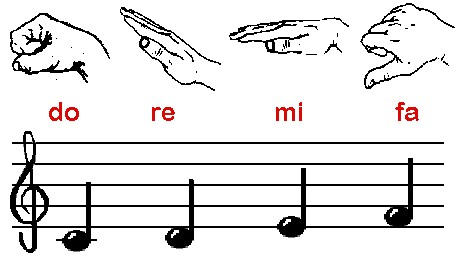
\includegraphics[width=0.45\linewidth]{figures/doremifa.jpg}
	}
	\hspace{0.03\linewidth}
	\subfloat{
		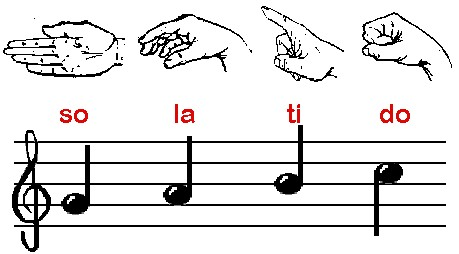
\includegraphics[width=0.45\linewidth]{figures/solatido.jpg}
	}
	\caption{The curwen hand symbols and the corresponding musical notes}
	\label{fig:curwennotes}
\end{figure}


\section{The Goal}
\label{sec:goal}
The goal of this thesis is to describe the design, build and evaluation process of a system for hand pose recognition. The system needs to be fast and user friendly; it should be able to run on current consumer hardware. Overall the system should satisfy the following requirements:

\begin{itemize}
	\item Extract a set of hands in video
	\item Extract position of hands in video
	\item Real time performance (10+ fps)
	\item Normal consumer processing power
	\item Normal RGB camera (webcam)
	\item No gloves or skin mounted electromechanical sensors
	\item No calibration or initialization
	\item Minimal configuration/parameters
\end{itemize}
	
To realize these requirements some restrictions on the system's setting are required:

\begin{itemize}
	\item One person in the image
	\item Person is wearing clothing with long sleeves
	\item Good enough lightning conditions
	\item No skin like colors in the image
\end{itemize}

The system can be used as a controller for a computer, with a focus on subtile detail for continuous variables, which give the sence of more direct control - important for real time interaction. Just how a graphical designer prefers a graphics tablet over a mouse for drawing, the design of the system aims to accomplish a similar sensation. The output of the system can be easily configured by a user to map to his or her preferred set commands. For example one hand control the pitch of a sound, while the other controls a accompanying beat while the position of this hand controls a cutoff filter. 

It is important to say that the scope of this thesis is limited to extracting the hand poses from video, and will not cover the study of the mapping of hand poses into sound. Although a prototype system is published along this thesis.



\section{Related Work}
At the moment of writing this thesis Microsoft is finishing the development of a new commercial product called 'Kinect'. Kinect is claimed to provide full-body 3D motion capture. To accomplish this, Kinect uses a range camera, which interprets 3D scene information from a continuously-projected infrared pattern. For this setting an infrared projector and a range camera is required. It is interesting to see that again (this is also the case for the Wii) a new revolutionary input device is created for a gaming console. 

\begin{figure}[htbp]
	\center{}
	\label{fig:kinect}
	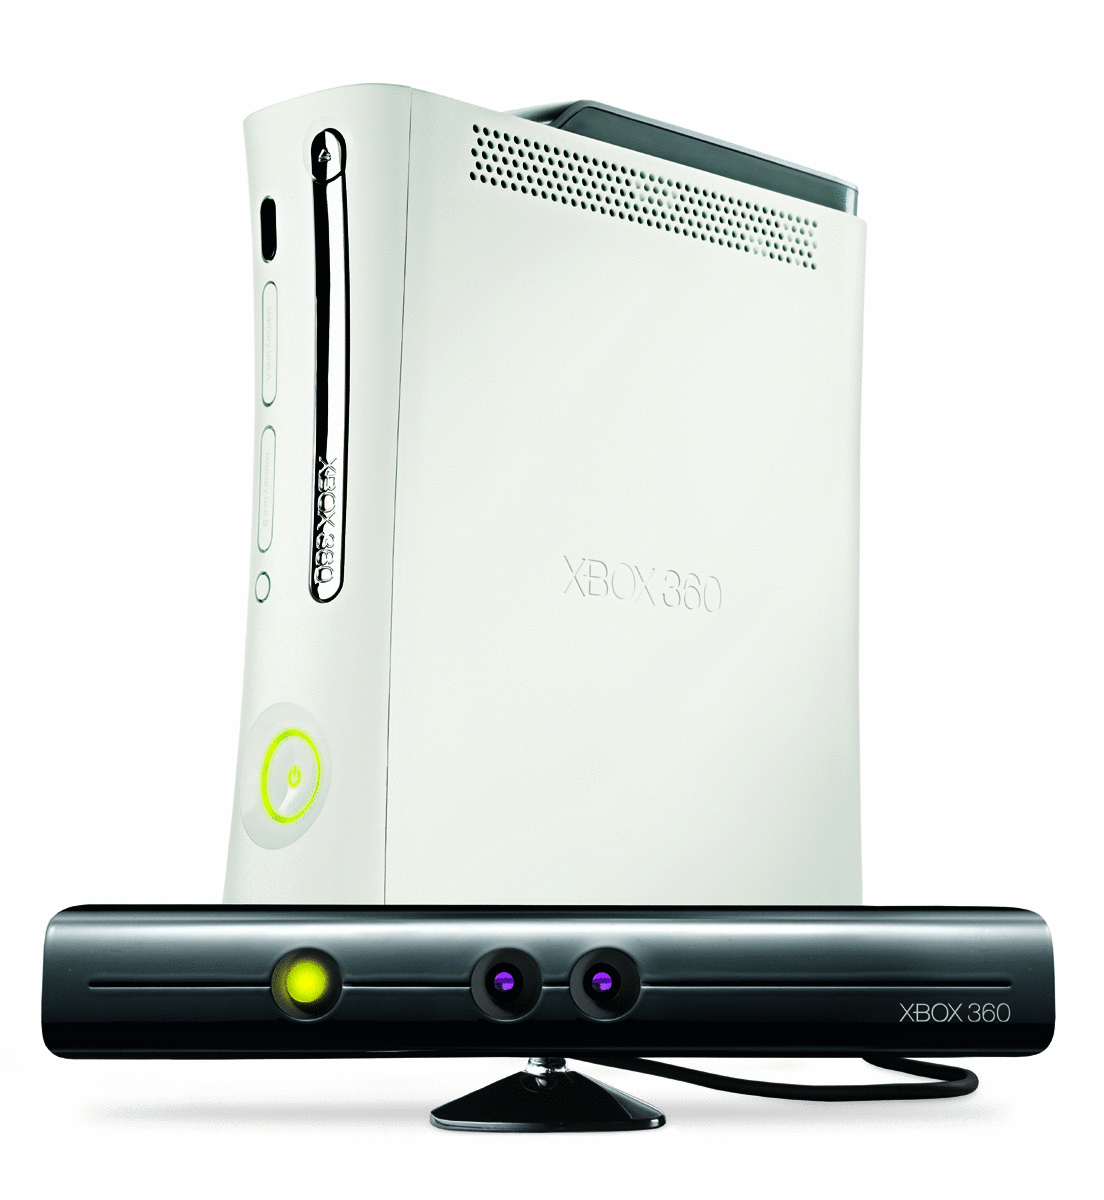
\includegraphics[width=0.3\linewidth]{figures/wave.jpg}
	\caption{Microsoft Kinect}
\end{figure}


An other interesting development is \cite{Wang2009} where a colored glove is used to perform full 3d hand pose estimation which seem to yield promising results. The disadvantage of this method is the intrusive requirement of wearing a specific color glove. 

\begin{figure}[htbp]
	\center{}
	\label{fig:wang2009}
	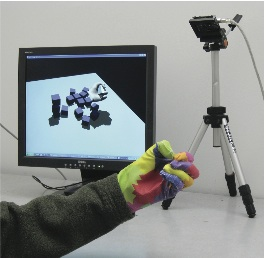
\includegraphics[width=0.4\linewidth]{figures/wang2009.jpg}
	\caption{3D hand pose estimation using a colored glove}
\end{figure}




Similar research has been done \cite{Wang2007}. Here SIFT features are used to discriminate 3 different hand symbols. A performance of 95.6\% is claimed using a the 'sharing feature concept'.


Research has been done in automated sign language interpretation using computer vision\cite{Buehler2009}\cite{RichardBowden2004}. The problem with interpreting sign language is a very large vocabulary, segmentation of the different gestures and representing the gestures in a robust way.

\cite{Yi2009} proposed a method for computer aided 3d architecture design using hand gestures, see \autoref{fig:yi2009} for the a model constructed with this software.

\begin{figure}[htbp]
	\center{}
	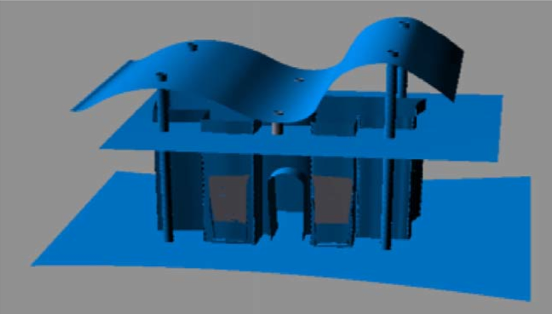
\includegraphics[width=0.6\linewidth]{figures/yi2009.png}
	\caption{3D model of train station made with aid of hand gestures}
	\label{fig:yi2009}
\end{figure}


\paragraph{Body Poses}
2d human pose estimation in tv shows \cite{ferrari2008},
advances in vision based hum motion capture and analysis (survey) \cite{Moeslund2006},
Vision-based human motion analysis (overview) \cite{Poppe2007},
Real-Time Body Pose Recognition using 2D or 3D haarlets \cite{VandenBergh2009}

\paragraph{hand Gestures}
Estimating 3d hand pose from a cluttered image \cite{Athitsos2003},
A very old paper using hand motion for segmentation \cite{Cui1996},
Vision-based hand pose estimation (Review): \cite{Erol2007},
A variational approach to monocular hand-pose estimation \cite{laGorce2010},
Old paper using shadows to estimate 3d hand pose \cite{Segen1999},
A PhD thesis exploring the hand as a input device \cite{Sturman1992},
Gesture recognition (survey) \cite{Mitra2007},
Real-time hand pose recognition using low-resolution depth images \cite{Mo2006},
visual recognition of pointing gestures for robot interaction \cite{Nickel2007},
Template-based hand pose recognition using multiple clues \cite{Stenger2006},
whole-hand input \cite{Sturman1992},
pixel based hand pose recognition using SIFT features \cite{Wang2007},
hand gesture extracting using adaptive skin color models \cite{Xiong2006},

\paragraph{Sign Language}
Learning sign language by watching TV using weakly aligned subtitles \cite{Buehler2009},
Large lexicon detection of sign language \cite{Cooper2007},
A linguistic feature vector for the visual interpretation of sign language \cite{RichardBowden2004}




An interesting overview paper is \cite{Erol2007}, which reviews the current state, possibilities and limitations of computer vision based hand pose and gesture recognition.



